\section{Porovnání dostupných CRM řešení} 
%%%%%%%%%%%%%%%%%%%%%%%%%%%%
V současné době je dostupných CRM řešení na trhu \uv{jak hub po dešti}. 

Během krátkého hledání na internetu, pomocí klíčových slov \uv{best CRM systems 2022}, narazíme na články \cite{PCMagCRM2022}\cite{TechRadarCRM2022} o nejlepších CRM systémech tohoto roku a zjistíme, že nejlépe hodnocené systémy, se ve svých vlastnostech navzájem moc neliší. Tyto články vyzdvihují systémy Salesforce Sales Cloud, Freshsales CRM, Zoho CRM, HubSpot CRM, Zendesk Sell nebo Apptivo CRM. 

Všechny podporují podobné funkcionality: evidence zákazníků, automatizace procesů, mobilní verze, vytváření reportů a do jisté míry i vlastní customizace. Tyto CRM systémy často přesahují i do taktických a strategických procesů podniku.

Tyto články malým podnikům doporučují například systém HubSpot CRM \cite{PCMagCRM2022} ale, nejen kvůli zadání této práce, nelze ignorovat Salesforce. Ten je již osm let největším hráčem na trhu s CRM řešeními. \cite{SalesforceCRMmarketShare}
%%%%%%%%%%%%%%%%%%%%%%%%%%%%
\subsection{Salesforce, Inc.} \label{SalesforceCRM}
Americká společnost Salesforce, se sídlem v San Franciscu, působí na trhu s cloudovým softwarem již od roku 1999. Zaměřuje se na poskytování cloudových softwarových produktů a služeb v oblasti CRM. \cite{SalesforceHistory}

Své produkty nabízí jako SaaS (Software-as-a-Service) a PaaS (Platform-as-a-Service), tím svým zákazníkům šetří starosti s hardwarem a infrastrukturou.

Pro lepší představu rozdílu mezi On-Site, IaaS (Infrastructure-as-a-service), PaaS a SaaS systémy se můžeme podívat na následující obrázek \ref{fig:IaasPaasSaas}.
Z tohoto obrázku je dobře vidět, že v případech PaaS a SaaS systémů jsou požadavky na vlastní hardware minimální. Tím se vstupní investice do provozu informačního systému snižuje.

\begin{figure}[!h]
    \centering
    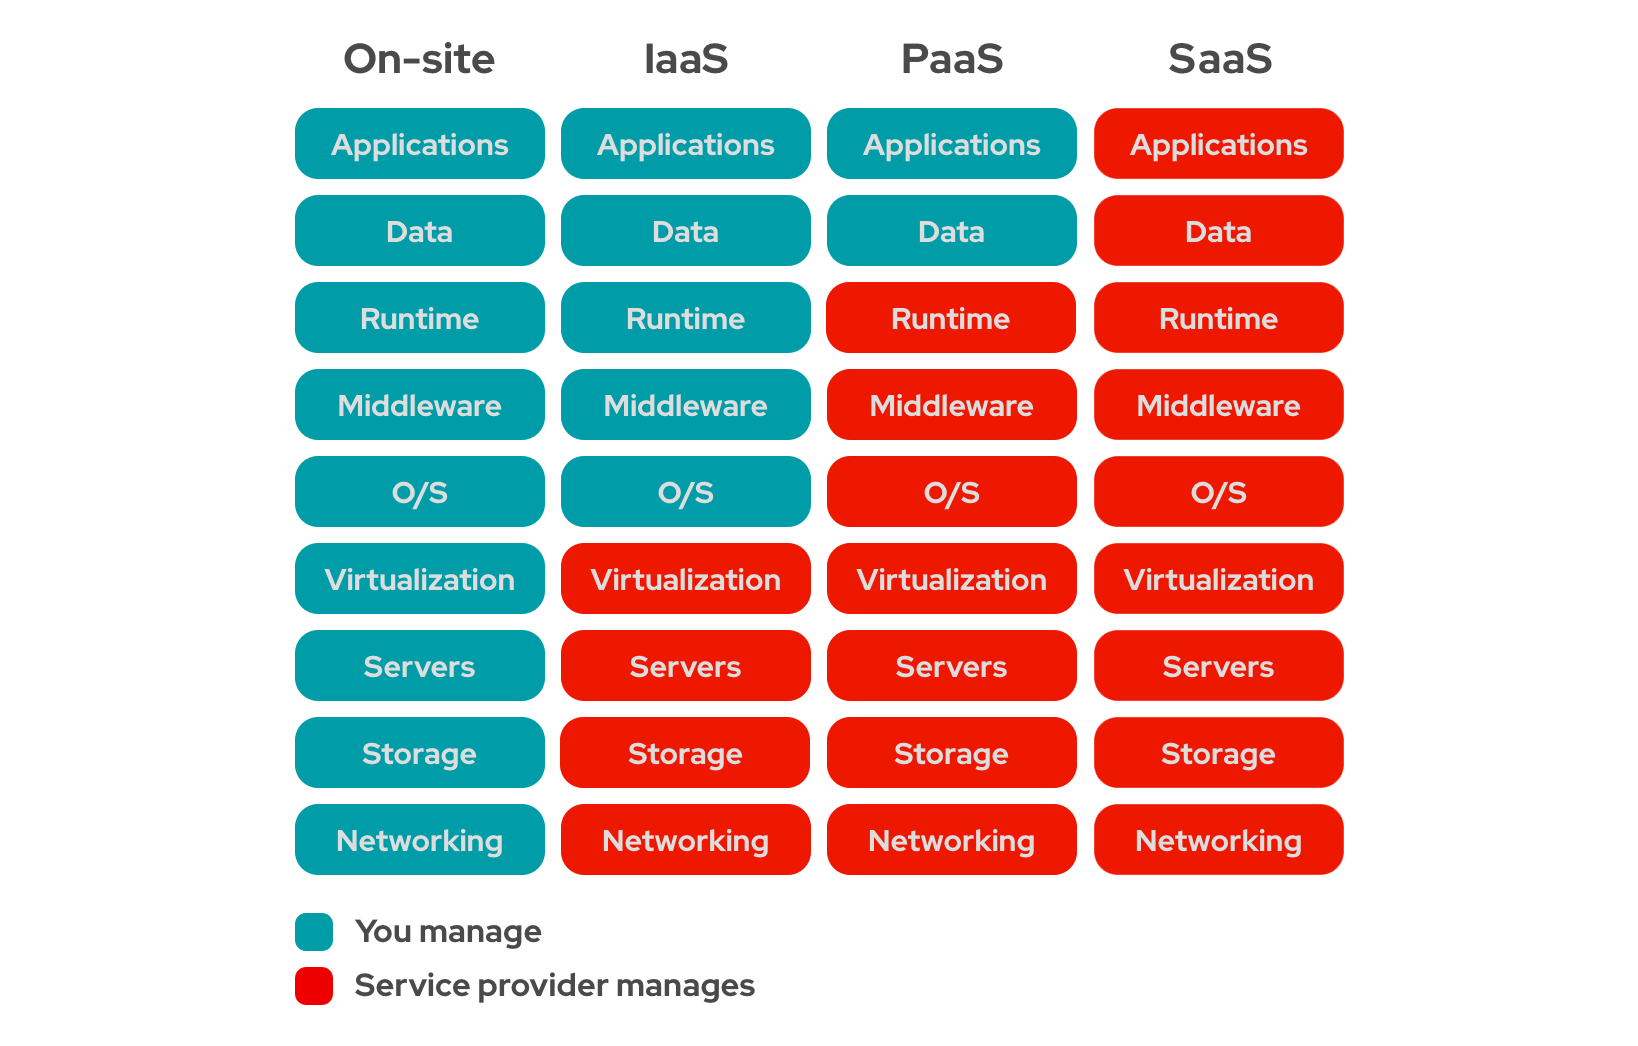
\includegraphics[width=\textwidth]{assets/2_IS/iaas-paas-saas-diagram.png}
    \caption[Diagram rozdílů výpočetních prostředí.]{Diagram rozdílů výpočetních prostředí. \cite{RedHatIaasPaasSaas}}
    \label{fig:IaasPaasSaas}
\end{figure}
\FloatBarrier
%%%%%%%%%%%%%%%%%%%%%%%%%%%%
\subsubsection{Produkty Salesforce}
Společnost Salesforce nabízí široké množství produktů a služeb, mezi nejznámější patří:
\begin{description}
    \item [Sales Cloud] je jejich CRM řešení pro podporu prodeje.
    \item [Service Cloud] je software na podporu zákaznického helpdesku.
    \item [Marketing Cloud] je služba podporující rozesílání marketingových emailů.
    \item [Comunity Cloud] slouží k podpoře zákaznických komunit.
    \item [Einstein Analytics] nabízí tvorbu analýz a podporu Business Inteligence pomocí umělé inteligence.
    \item [Platform] je služba zaměřená na tvorbu vlastních aplikací na platformě Salesforce.
\end{description}

Salesforce si udržuje i vlastní obchod s aplikacemi AppExchange, který, díky velikosti Salesforce komunity, je plný aplikací, komponent a funkčností připravených k integraci. Skrze tento obchod mohou další společnosti propojovat svoje služby s aplikacemi Salesforce. \cite{PCMagSalesforceReview}

Salesforce většinu svých produktů poskytuje v několika úrovních licencí, které se liší cenou a dostupnými funkcemi. Ceny služeb se pohybují od \texteuro{25} za uživatele na měsíc \cite{SalesforcePricing}, další úrovně se u jednotlivých služeb liší. Kompletní seznam služeb a porovnání edic je k dispozici na jejich webu.
%%%%%%%%%%%%%%%%%%%%%%%%%%%%
\subsubsection{Salesforce pro malé podniky}
Salesforce malým podnikům nabízí balíčky obsahující služby Sales Cloud, Service Cloud a Marketing Cloud. Ceny těchto balíčků se pohybují od zmíněných \texteuro{25}. 

Konkrétně Sales Cloud pro podporu prodeje, je v této nejlevnější edici Essentials velmi omezený, například nepodporuje vytváření vlastních objektů a aplikací. 

Kompletní přehled edic Sales Cloudu a funkcí je k dispozici na webu. \cite{SalesforcePricingSalesCloud}

Pro některé podniky je potřebná tvorba vlastních objektů a aplikací, tyto funkce jsou dostupné od edice Professional, která se cenově pohybuje od \texteuro{75} za měsíc za uživatele. \cite{SalesforceCustomObjectLimit}

Hlavní překážkou nejlevnější edice je ta, že podnik se musí přizpůsobit tomuto systému a naučit se s ním pracovat. V dražších edicích Professional a Enterprise se možnosti vlastní customizace drasticky zvyšují a systém lze přizpůsobit podniku.
